\documentclass{eplDoc}

\usepackage{placeins}

\newcommand{\docType}	{Assignment 1 : Markov Decision Processes}
\newcommand{\docDate}	{16/03/2012}
\newcommand{\docAuthor}	{gr10 : Mulders Corentin, Pelsser Francois}
\newcommand{\courseCode}{SINF2275}
\newcommand{\courseName}{Data mining and decision making}
\usepackage{syntax}

\lstset{breaklines=true, breakatwhitespace=false}

\begin{document}
\maketitle
\newpage

\section{Method used to determine the optimal strategy}

\subsection{Brief description of the method}
To select the dice to throw in the current state we use a markov decision process. To do this we had to define a way to represent the problem and implement the markov process itself. 

\subsubsection{Representation of the problem}
We define the state of the game as the number of the square on wich the player is. At each state the only two possible actions are to throw the security or the risky dices. Our actions all have a fixed cost of $1$ independently of the state (this is only true if there are no prison squares, when we add those they lead to some actions having a cost of $2$ as it will be explained later). \\ 
We represent the game board as an affinity matrix, its elements are : 
\begin{itemize}
	\item $a_{ij}=0$ if the player can't move from i to j in one step.
	\item $a_{ij}=1$ if the player goes from i to j following the main path.
	\item $a_{ij}=2$ if the player goes from i to j following a secondary path.
\end{itemize}
The initial state and goal state values are also stored each in a variable. \\ 
In addition to this we have the vector List received as argument that defines the types of squares. \\ 

\subsubsection{Markov decision process}
We use the value iteration algorithm to compute the optimal expected cost. 

%todo, je pige pas trop ce qu'on fait en fait




\subsection{Additional experiments}


\subsubsection{Prison squares}

If a case is a prison square and the player stops on it when using the risky dice then the cost of the action is $2$ instead of $1$. This is because the consequence sof stopping on such a case is that a turn will be lost. So we can consider that to go on the case we need to throw the dice twice instead of once. 

\subsubsection{retreat squares}

If a case $i$ is a retreat square then if there is a probability $p$ to stop on this case. The probability to stop on this case becomes $0$ and there is a probability $p$ to get on the  $i-2$ square (or square $1$ if $(i-2)<1$). Off course that is only the cas eif the dice played was the risky dice. 


\subsubsection{Adaptation to any kind of of Snakes and ladders game}

Since the game board is represented as an affinity matrix it is very easy to use our implementation to play on a different board. The only thing to do is to define the affinity matrix corresponding to the new game and fetch it to the program. Off course the vectors of the traps types must also be adapted to match the number of squares in the game. \\ 
As an example of this functionality we designed a more complex game board and used it with our program. A representation of this new game board is shown below (arrows with interrupted lines represent secondary paths): 

\FloatBarrier
\begin{figure}%
	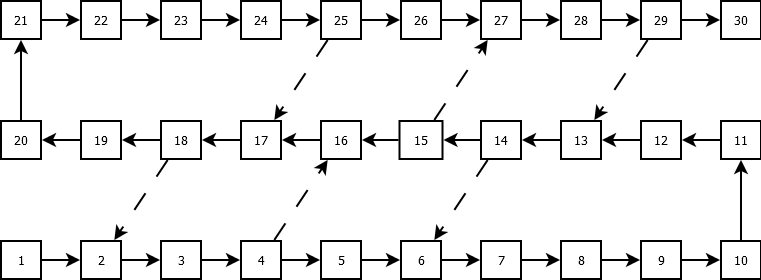
\includegraphics[width=\columnwidth]{newboard.png}%
	\caption{Complex board}%
	\label{newboard}%
\end{figure}
\FloatBarrier
 \ \\ 
%This board will be used as well as the basic board for the analisys of our results compared to a naive strategy. 

%\subsubsection{Use of reinforcement learning}


\section{Results obtained with our implementation}

We used octave to write our implementation of \textbf{[Expec, Dice] = markovDec(list)}. We compare our decision process with three naive policies :
 
\begin{description}
	\item[Security] always plays the security dice.
	\item[Risky] always plays the risky dice.
	\item[Random] has a $50\%$ probability to play either of the dices.
\end{description}


\end{document}
